%Document Class
\documentclass[twocolappendix]{latex/emulateapj}

%Packages and Commands
%PACKAGES
\usepackage{multirow,color,wrapfig,ulem}
\usepackage {graphicx}
\usepackage{amsmath}
\usepackage[dvips]{epsfig}
\usepackage{fancyhdr}
\usepackage{epsfig}
\usepackage{graphicx}
\usepackage{amsmath}
\usepackage{amssymb}
\usepackage{latexsym}
\usepackage{epic}
\usepackage{hyperref}

%COMMANDS
\newcommand{\Msun}{{\ifmmode{{\rm {M_{\odot}}}}\else{${\rm{M_{\odot}}}$}\fi}}
\newcommand{\kms}{{\ifmmode{{\mathrm{\,km\ s}^{-1}}}\else{\,km~s$^{-1}$}\fi}}
\newcommand{\lya}{{Ly-$\alpha$~}}

\newcommand{\tauh}{{$\tau_{\rm H}$~}}
\newcommand{\vrot}{{$v_{\rm rot}$~}}
\newcommand{\vout}{{$v_{\rm out}$~}}

\newcommand{\ang}{{$\theta_{gal}$~}}
\newcommand{\lognh}{{$\log{n_H}$~}}
\newcommand{\nh}{{$n_H$~}}

\begin{document}

\title{Influence of galaxy rotation and outflows in the Lyman Alpha spectral line}
\shorttitle{Influence of galaxy rotation and outflows in the Lyman Alpha spectral line}

\shortauthors{Remolina-Gutierrez et al.}

\author{Maria Camila Remolina-Gutierrez, Jaime E. Forero-Romero} 
\affil{Departamento de F\'{i}sica, Universidad de los Andes, Cra. 1 No. 18A-10, Edificio Ip, Bogot\'a, Colombia}
\email{mc.remolina197@uniandes.edu.co}
\email{je.forero@uniandes.edu.co}

\keywords{Galaxies: high-redshift, Lyman Alpha Emission, Galaxy Rotation, Galaxy Outflows, Radiative Transfer}  

\begin{abstract}
\noindent Young galaxies in the Universe have a strong \lya emission caused by the ionized Hydrogen atoms in their interstellar medium. When the spectrum of a galaxy has an intense peak around the \lya natural frequency ($2.46\times 10^{15}$ Hz) it is called a Lyman Alpha Emitter (LAE). Typical LAEs are very distant ($z \gtrsim 2$). This makes that all the data astronomers can obtain from them is their spectra, and from there all the physical information of the galaxy must be derived. Trying to solve this task requires the creation of a simplified and solid model. In this paper we propose to consider LAEs as a spherical distribution of Hydrogen atoms that undergoes a solid body rotation and a radial expansion due to outflows. We use radiative transfer Monte Carlo simulations to interpret the Lyman-$\alpha$ line morphology. The main conclusion is that this new model reproduces LAEs observed features in a clear way and with consistent physical parameters. We also show results of adjusting observational data for some selected objects to models with and without bulk rotation. We finalize by discussing the possible implications for these results in terms of the energetics required for supernova feedback and outflows in high redshift galaxies. \\
\end{abstract}

\section{Introduction}
\label{sec:intro}

Galaxies are key to understand our Universe. However, distant ones are very challenging to detect. It is then an open challenge to obtain as much information as possible from them, as they represent the younger stages of galaxy evolution. Astronomers noted that a that relevant fraction of these galaxies emitted a really strong line at $1215.67\;\AA$ in their spectra at  and named them Lyman Alpha Emitters (LAEs). The purpose of this paper is to use this spectral line to model and simulate LAEs in order to narrow computationally their physical and kinematic properties. \\

In the early Universe the most abundant elements were Hydrogen(H) and Helium(He), causing young galaxies to be rich in H atoms. Due to stellar activity in a galaxy, the surrounding gas is ionized, so H atoms excite and emit radiation at definite frequencies. The most basic of these frequencies corresponds to the \lya line equal to $2.47 \times 10^{15}\;Hz$ \cite{PartridgePeebles}. This is equivalent to a wavelength of 1215.67 $\AA$ cause by the transition of the H atom electron from levels $2\rightarrow1$ dubbed Lyman Alpha ( \lya) transition, discovered by Theodore Lyman in 1906. \cite{LymanBio} \\

Due to the amount of H atoms inside a galaxy, the whole body becomes a strong \lya radiator. If the galaxy spectra shows a strong \lya line, it classifies as a Lyman Alpha Emitter (LAE). (\cite{DjorgovskiThompson}, \cite{Rhoads00}, \cite{Gawiser2007}, \cite{Koehler2007}, \cite{Ouchi08}, \cite{Yamada2012}, \cite{Schenker2012}, \cite{Kulas12}, \cite{Yamada2012}, \cite{Chonis2013}, \cite{Finkelstein2013}, \cite{Ostlin14}, \cite{Hayes2014}, \cite{Faisst2014}, \cite{Fumagalli2015}). However, when a \lya photon is emitted inside the galaxy, it travels through its interstellar medium (ISM). During the photon's path it can be absorbed and re-emitted by other H atoms. The new frequency of the photon is different that the initial one, in an observer frame of reference due to the atom's velocity. In LAEs, the state of the ISM gas, before and after a photon's re-emission is pretty much the same. This allows a random walk approximation and lets us consider photon-atom encounters as scatterings. A photon's scattering can happen several times, as seen in Fig. \ref{fig:radiative_transfer}. This stops only until the photon is able to escape the galaxy. \\

\begin{figure}[h!]
	\begin{center}
		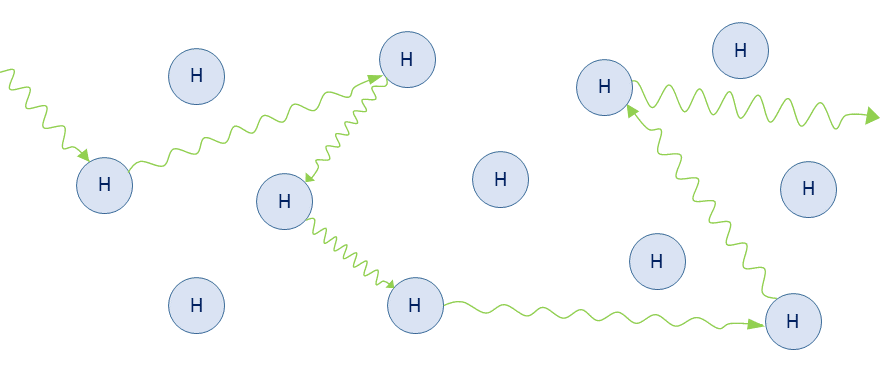
\includegraphics[width=0.45\textwidth]{./figures/radiative_transfer}
	\end{center}
	\caption{\textbf{Radiative Transfer Sketch:} A \lya photon being absorbed and re-emitted by Hydrogen atoms. 
		\label{fig:radiative_transfer}}
\end{figure}

In a static galaxy, this random walk process produces a spectrum with two equal and symmetric peaks around the natural \lya wavelength. This can be seen in Figure A3 of Forero-Romero et al. paper \cite{CLARA} (Fig. \ref{fig:static}). If now the gas has a bulk velocity, the shape of the \lya profile changes. We explore these effects in this paper by proposing a new model for a LAE. The model consists of a spherical distribution of H atoms undergoing a solid body rotation and radial expansion (outflows). \\

\begin{figure}[h!]
	\begin{center}
		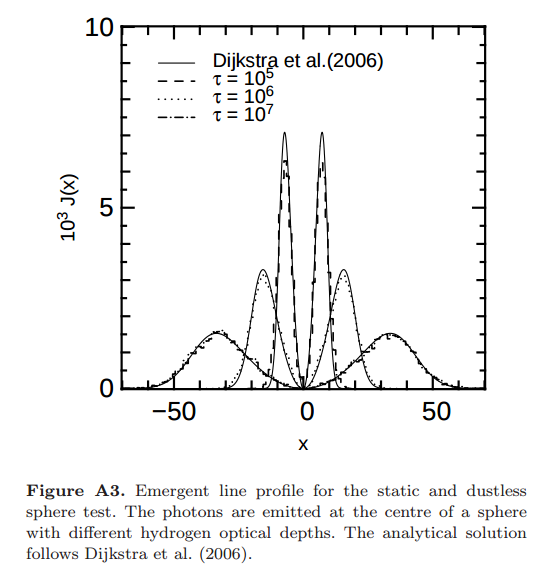
\includegraphics[width=0.35\textwidth]{./figures/static}
	\end{center}
	\caption{\textbf{Figure A3 of Forero-Romero et al. paper:} CLARA's view on the escape fraction of Lyman-$\alpha$ photons in high redshift galaxies \cite{CLARA}. Reproduced with the permission of the author.
		\label{fig:static}}
\end{figure}

Our main goal with this work is to measure the effect of the model's physical parameters on the outgoing \lya line. In this case, due to the resonant\footnote{Resonant is a common term used in radiative transfer. It means that the photons that create the line are absorbed and re-emitted several times before escaping the cloud of gas.} nature of the \lya line, analytical solutions can not be derived. Because of this, it becomes necessary to run simulations that explore and test the model. In this paper we use the radiative transfer code \textbf{CLARA} (Code for Lyman Alpha Radiation Analysis) written by Forero-Romero et al. \cite{CLARA}. CLARA can simulate the \lya line of a spherical rotating LAE depending on its mass and velocity, so we modify it to include outflows and then we explore the resulting consequences on the \lya line. \\


\section{A new LAE model}
\label{sec:newmodel}

We model spherical galaxy to facilitate the interpretation of the results, by deleting what would be another degree of freedom regarding a different geometry. Furthermore, this approximation is commonly used in the literature, as it explains a wide variety of observational features (\cite{Ahn03}, \cite{Verhamme06}, \cite{Dijkstra06}). \\

There are 3 parameters in this model that define a LAE: the rotational velocity (\vrot), the outflow velocity (\vout) and the optical depth (\tauh). \vout is due to material ejected from the galaxy, by supernovas(\cite{Verhamme06}, \cite{Orsi12}, \cite{Hashimoto2015}, \cite{Gronke2015}). \tauh roughly corresponds to number of H atoms found by a \lya photon if one traces a line from the center of the galaxy to its edge, and it resembles the mass of the LAE.\\

In this model, the LAE has a bulk velocity corresponding to the superposition of rotation and outflows, as shown in Fig. \ref{fig:model}. The velocity components are written in Eqs. (\ref{eq:vx}) (\ref{eq:vy}) (\ref{eq:vz}). In these equations, $R$ is the radius of the sphere; $x$, $y$ and $z$ are the coordinates in a cartesian frame; and the $\mp$ signs in $v_x$ and $v_y$ indicate the direction of rotation, respectively. This rotation is a solid body rotation and its direction goes according to the right hand rule applied to the $\hat{k}$ unit vector. The outflow velocity is dependent on the position relative to the center of the galaxy, being it zero at the center and maximum at the edge of the sphere.\\

\begin{equation}
	v_{x}=\frac{x}{R}v_{\rm out}-\frac{y}{R}v_{\rm rot} 
	\label{eq:vx}
\end{equation}

\begin{equation}
	v_{y}=\frac{y}{R}v_{\rm out}+\frac{x}{R}v_{\rm rot} 
	\label{eq:vy}
\end{equation}

\begin{equation}
	v_{z}=\frac{z}{R}v_{\rm out}
	\label{eq:vz}
\end{equation}

These 3 parameters, \vrot, \vout and \tauh, leave the idea of a model of LAE, that although simple, considers the main galaxy's dynamics. All of them have been previously proposed and used by different authors, but never combined together (\cite{Adams72}, \cite{Harrington73}, \cite{Neufeld90}, \cite{Dijkstra06}, \cite{Verhamme06}, \cite{Forero12}, \cite{Martin2015}, \cite{Garavito14}, \cite{Neufeld91}, \cite{Laursen09}, \cite{Barnes11}, \cite{Verhamme12}, \cite{Yajima12}).\\

\subsection{A \lya Photon's Path in CLARA}
\label{subsec:photons_path_clara}

In the \lya radiative transfer problem, a commonly used dimensionless variable $x$ is used to describe a photon's frequency and is defined as:\\

\begin{equation}
	\label{eq:x_freq}
	x \equiv \frac{\nu -\nu_{\rm \alpha}}{\Delta\nu_{\rm D}},
\end{equation} 

where $\nu$ is the photon's frequency and $\nu_{\rm \alpha} = 2.46\times 10^{15}$ Hz is the \lya natural frequency. The denominator $\Delta\nu_{\rm D}$ is defined in Eq. \ref{eq:delta_nuD}.

\begin{equation}
	\label{eq:delta_nuD}
	\Delta\nu_{\rm D} \equiv \nu_{\rm \alpha}\sqrt{\frac{2kT}{m_pc^2}} \equiv \nu_{\rm \alpha} \frac{v_{\rm th}}{c},
\end{equation} 

where $\Delta\nu_{\rm D}$ is known as the Doppler broadening of the \lya line. It depends on the neutral gas temperature $T$ or equivalently the thermal velocity $v_{\rm th}$ of the atoms. In the model the temperature is kept constant at $T=10^4$K and the thermal velocity is $v_{\rm th}=12.8$\kms. \\

If $x < 0$, the final frequency $\nu < \nu_{\rm \alpha}$. This translates to the final wavelength being larger than the \lya natural one, casing a redshift in frequency. If, on the contrary, $x > 0$, the photon suffers a blueshift in frequency. \\

However, in the plots shown in this paper we use instead velocity, $V$, units. This eases the comparison against observational data. The velocity units are defined by

\begin{equation}
	\label{eq:V}
	V = xv_{\rm th} = \frac{\nu -\nu_{\rm \alpha}}{\nu_{\rm \alpha}}c.
\end{equation}

The units of $V$ are usually \kms. In this case, the photon is redshifted in frequency when the velocity is greater than 0, and blueshifted in the opposite case. \\

The initial emission of photons is taken at the center of the sphere for practicality due to the fact that both, center and off-center emissions, give analogous results. From here, $100000$ photons are emitted with the natural \lya wavelength starting to behave as described in sub-section \ref{subsec:photons_path_clara} (See Fig. \ref{fig:radiative_transfer}). When each photon is re-emitted, its new wavelength depends on the H atom's velocity (both thermal and bulk) and direction (both initial and final). However the photon's new direction of propagation is random in the rest frame of the atom. \\ 

The individual scattering of all the photons is tracked through the complete 3D Hydrogen distribution. Once each photon escapes the galaxy, its final values are stored: position $\vec{r}$, direction of propagation $\hat{k}$, dimensionless frequency $x$, and number of scatterings $N$. To build the observed spectrum we make a histogram of the escape frequencies $x$. The number of scatterings $N$ tells how many steps the random walk requires to reach a distance to the center that is $\geq R$. In order to avoid situations in which the photon has not escaped after a long computational time, CLARA defines a number $N_{max}$ so the code stops. However, according to statistics, this last situation has low probabilities, so the photon is always most likely to exit the sphere. \\

%The process that takes place from the moment the first photon is emitted to the moment the last photon escapes the sphere, is called a simulation. Each simulation runs in the scientific computational cluster of Universidad de los Andes due to the computing resources it requires. Depending on \tauh, we need a different number of processors in order to minimize the time demands. For \tauh $=10^5, 10^6, 10^7$ we use 6, 12, 24 processors, respectively. The running times go from 7 hours to 1 week approximately, depending on the case. \\

\subsection{Galaxy's Viewing Angle}
An observer located far away, only receives photons emitted along its line of sight. That means, only photons escaping in the direction of the observer must be counted in the spectrum. In the simulation we approximate this by taking into account only the photons with escaping direction angle $\theta$ respect to the rotation axis within the range $[\theta_{min}-\theta_{max}]$. We illustrate this in Fig. \ref{fig:model}. \\

\begin{figure}[h!]
	\begin{center}
		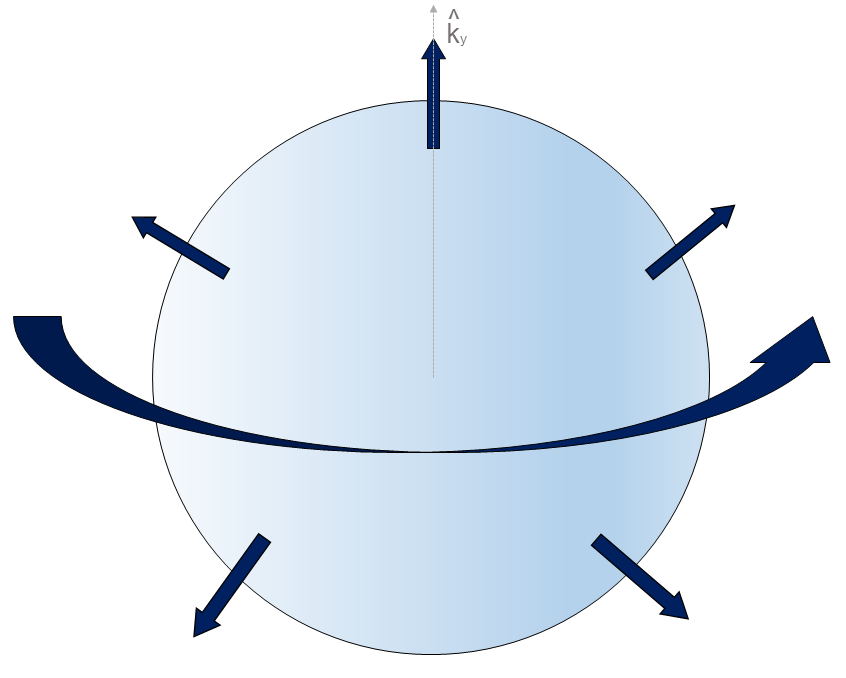
\includegraphics[width=0.48\textwidth]{./figures/model}
	\end{center}
	\caption{\textbf{Model:} Spherical LAE with tangential and radial velocities due to rotation and outflows, respectively. The galaxy cut is in the $y-z$ plane perspective. The observer is located at an specific viewing angle of the sphere. Only photons with a direction that enters in this range of vision are taken into account to build the observed spectrum.
		\label{fig:model}}
\end{figure}

Therefore, in principle the spectra depend on two new parameters, the azimuthal and the polar angle. However, the galaxy's motion is symmetrical respect to its rotation axis. This implies that the resulting spectrum is independent from the azimuthal angle. Taking into account this symmetry, we only select photons on their polar angle, regardless of their azimuthal angle. Regarding the polar angle, we build the spectra for observers located on 3 different positions, with $\theta$ intervals uniformly distributed in $\cos(\theta)$. \\ 

To summarize, the parameters influencing the spectra are \vrot, \vout, \tauh and $\theta$. In the next section we evaluate the impact each of these has on the resulting profile. \\


\section{Results}
\label{sec:results}

\subsection{Parameters' Initial Values}
In order to define the ranges of \tauh, \vrot and \vout, it is necessary to refer to observational constraints. The common values for typical LAEs are in Tab. \ref{tab:values}. We run CLARA's modified version for all the permutations of these 3 parameters. \\

\begin{table}[htbp]
	\centering
	\begin{tabular}{|c|c|c|}
		\hline
		$\tau_{\mathrm{H}}$ & $v_{rot}$ (\kms) & $v_{out}$ (\kms) \\
		\hline
		$10^5$, $10^6$, $10^7$ & 50, 100 & 5, 10, 15, 20, 25, 50, 75 \\
		\hline
	\end{tabular}
	\caption{\textbf{Parameters' Values:} All consistent with a LAE's typical properties}
	\label{tab:values}
\end{table}

The resulting sets of spectra are in the Appendix \ref{ap:results_figures} in Figs. \ref{fig:3_tau10E5_phi83-90}, \ref{fig:3_tau10E7_phi83-90} and \ref{fig:3_tau10E6_phi83-90} for $\theta \simeq 90^\circ$. We do not include the spectra for \vout = 50, 75 \kms because they are similar to \vout = 25 \kms. For this reason, we limit \vout to a maximum value of 25 \kms in all the plots. Nevertheless, the figures for \vout = 50, 75 \kms are in the Appendix \ref{ap:additional_figures} in Figs. \ref{fig:2_tau10E5_phi83-90}, \ref{fig:2_tau10E6_phi83-90} and \ref{fig:2_tau10E7_phi83-90}.\\

These last 3 plots show a clear creation of two asymmetric peaks around $V=0$ \kms with the tallest peak is always redshifted, with a strong dependence on the outflow velocity.\\

\subsection{Influence of the viewing angle $\theta$}
We take now into account the viewing angle of the galaxy to build the observed spectra. For all of the physical parameters' combinations, the effect of $\theta$ in the \lya line is always the same.\\

\begin{figure}[h!]
	\begin{center}
		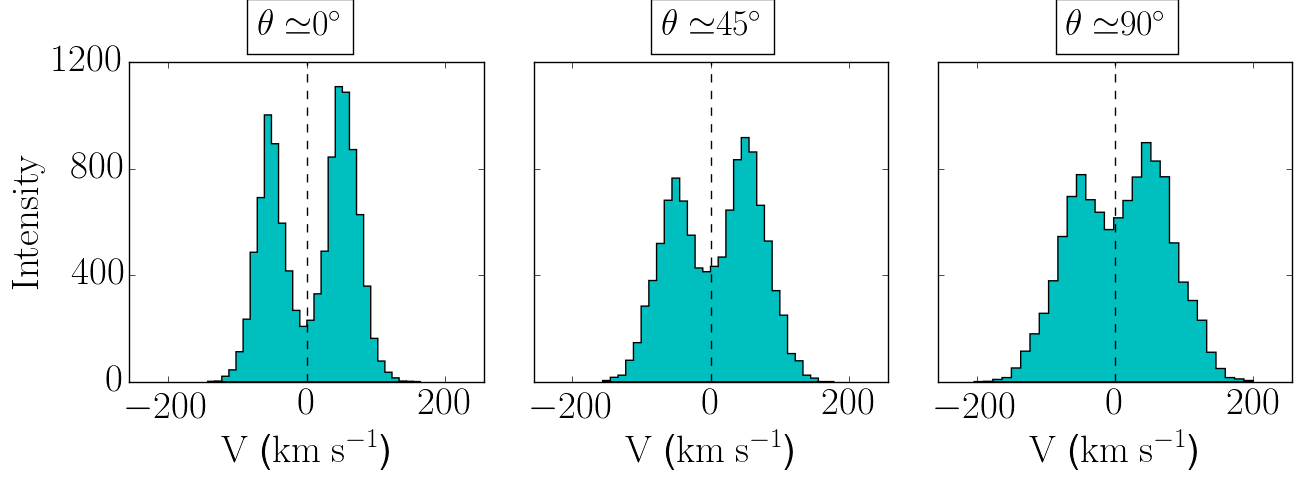
\includegraphics[width=0.5\textwidth]{./figures/influence_viewing_angle_5}
	\end{center}
	\caption{\textbf{\lya profile for different $\theta$:} With \tauh$=10^5$, \vrot$=50$ \kms and \vout$=20$ \kms.The intensity is in arbitrary units.
		\label{fig:influence_viewing_angle_5}}
\end{figure}

\begin{figure}[h!]
	\begin{center}
		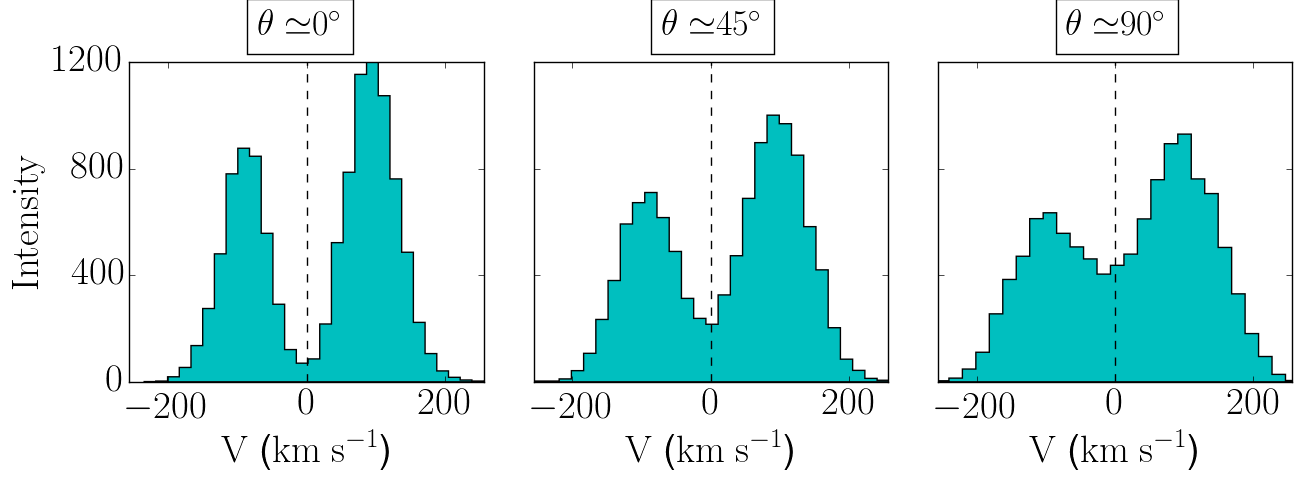
\includegraphics[width=0.5\textwidth]{./figures/influence_viewing_angle_6}
	\end{center}
	\caption{\textbf{\lya profile for different $\theta$:} With \tauh$=10^6$, \vrot$=100$ \kms and \vout$=5$ \kms.The intensity is in arbitrary units.
		\label{fig:influence_viewing_angle_6}}
\end{figure}

\begin{figure}[h!]
	\begin{center}
		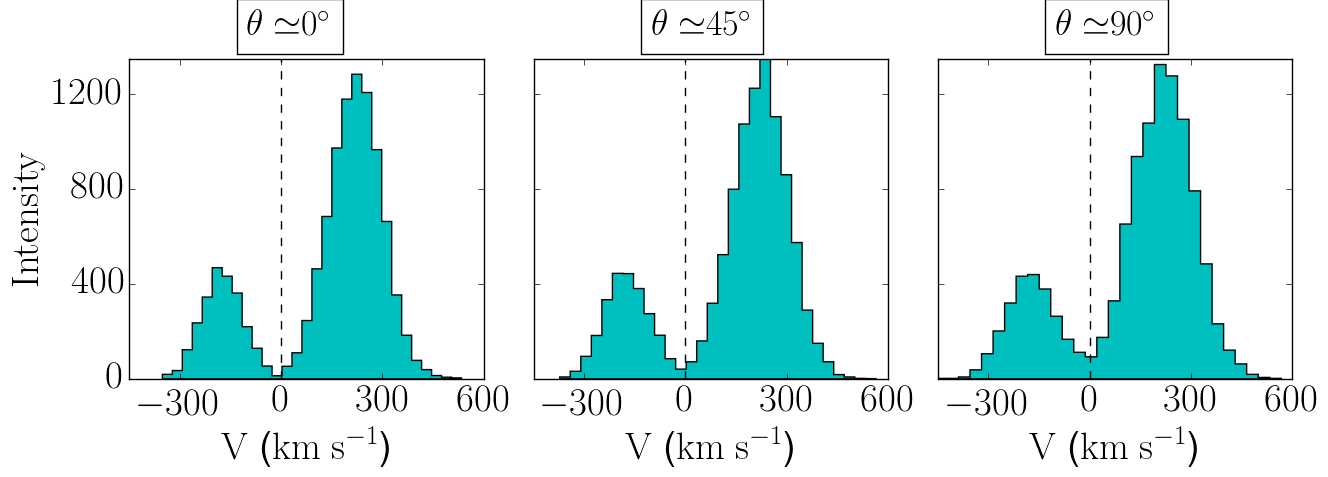
\includegraphics[width=0.5\textwidth]{./figures/influence_viewing_angle_7}
	\end{center}
	\caption{\textbf{\lya profile for different $\theta$:} With \tauh$=10^7$, \vrot$=100$ \kms and \vout$=15$ \kms.The intensity is in arbitrary units.
		\label{fig:influence_viewing_angle_7}}
\end{figure}

From Figs. \ref{fig:influence_viewing_angle_5}, \ref{fig:influence_viewing_angle_6} and \ref{fig:influence_viewing_angle_7} is clear that the intensity of the valley between the two peaks increases along with $\theta$. This causes an intensity decrease in the rest of the frequencies, thus a broadening of the line. The asymmetry also changes with the viewing angle.\\

In the next subsection, we show only the results of the angle at which an observer sees the galaxy's angular momentum vector perpendicular to the line of sight. The purpose of this is only to decrease the number of plots as there is an analogous behavior for all viewing angles. \\

\subsection{Morphology of \lya line}
To quantify the morphology of the \lya profile, we use an asymmetric gaussian fit to the curve as seen in Fig. \ref{fig:asymmetric_gaussian_fit}. Each of the two peaks, the red one and the blue one, is fitted with a curve parametrized by: an amplitude $A_{\pm}$, a standard deviation $\sigma_{\pm}$, a center $c_{\pm}$ and a skewness factor $\gamma_{\pm}$.\\

\begin{figure}[h!]
	\begin{center}
		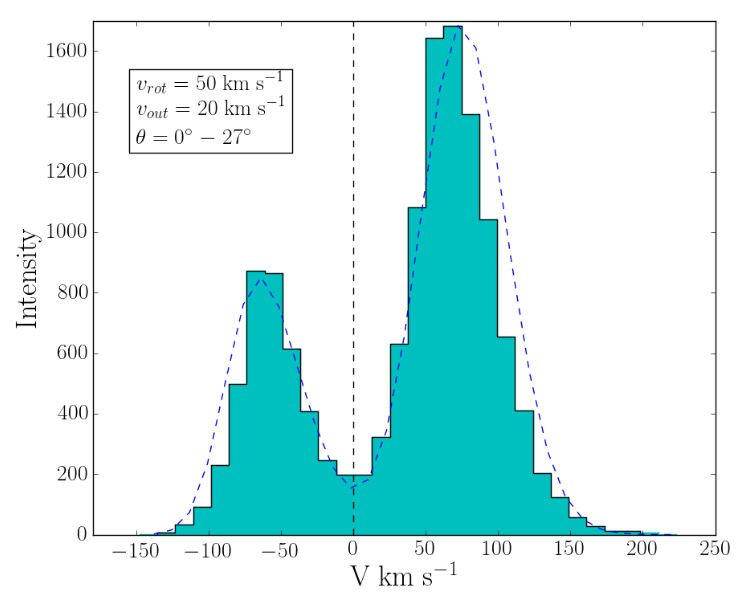
\includegraphics[width=0.3\textwidth]{./figures/asymmetric_gaussian_fit}
	\end{center}
	\caption{\textbf{Asymmetric gaussian fit for a \lya profile:} With \tauh$=10^5$, \vrot$=50$ \kms, \vout$=20$ \kms and $\theta \approx 0^\circ$.The intensity is in arbitrary units.
		\label{fig:asymmetric_gaussian_fit}}
\end{figure}

TERMINAR...\\


\subsection{Influences of the free parameters}

TERMINAR...\\

\begin{figure}[h!]
	\begin{center}
		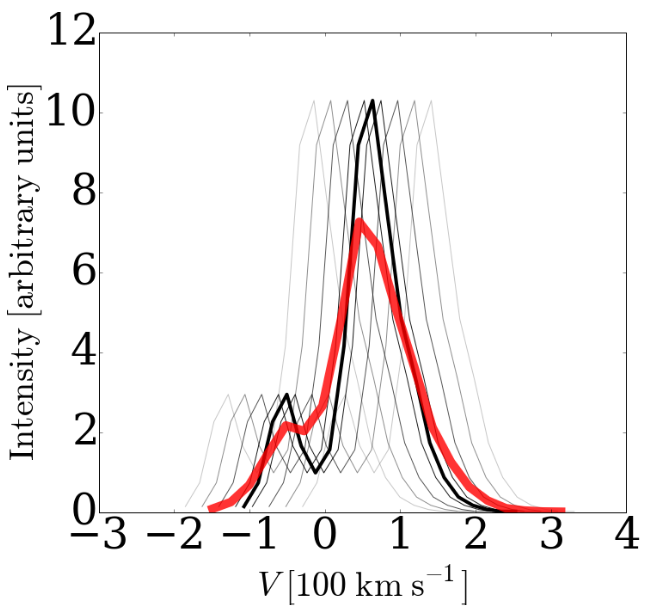
\includegraphics[width=0.3\textwidth]{./figures/rotation_doppler_outflow}
	\end{center}
	\caption{\textbf{Rotations induces a Doppler shift of the only-outflow spectra:} Each of the black lines is then weighted to obtain the red line.
		\label{fig:rotation_doppler_outflow}}
\end{figure}

To summarize the influence of the 3 parameters on the \lya morphology is the following: 

\begin{itemize}
	\item \tauh induces a redshift. Increasing the optical depth separates the line of the zero velocity line. \\
	\item \vout decreases the right peak's intensity. Higher \vout make the left peak smaller until it merges with the right one. \\
	\item \vrot broadens the line and decreases the maximum intensity. Higher \vrot implies a flatter spectrum. This effect has not been deeply studied in literature. Only Garavito et al. \cite{Garavito14} has simulated its effect. Our results are consistent with their conclusions. 
\end{itemize}

\section{Observational Comparison}
\label{sec:comparisonobservations}

There are several observations of LAEs in the literature. Kulas et al. \cite{Kulas12} observed distant LAEs ($z\sim2-3$) with high resolution. In the Figure 3 of their paper (Fig. \ref{fig:kulas}) they show 18 \lya profiles. \\

\begin{figure}[h!]
	\begin{center}
		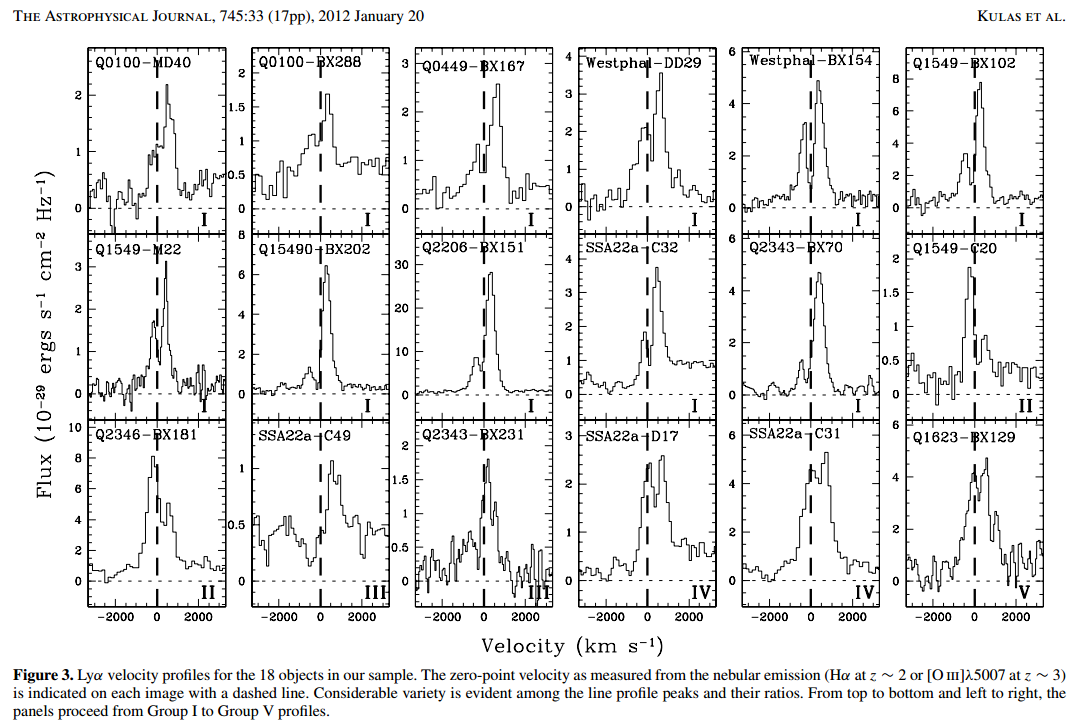
\includegraphics[width=0.5\textwidth]{./figures/figure3_kulas}
	\end{center}
	\caption{\textbf{Figure 3 of Kulas et al. paper:} The Kinematics of Multiple-peaked \lya Emission in Star-forming Galaxies at $z\sim2-3$ \cite{Kulas12}. This plot is reproduced with the authors permission.
		\label{fig:kulas}}
\end{figure}
%http://arohatgi.info/WebPlotDigitizer/app/

The observed spectra in Fig. \ref{fig:kulas} are modified by the redshift $z$ of the galaxies, which causes a broadening of the line. Taking into account this effect, we notice similitudes between them and the simulated spectra. The \lya profiles are mostly 2 peaks with an asymmetry between them, just as in the simulation. Also, the small peak (if existing) is always smaller than the tall one.\\

In this section we will focus in one particular observation from Fig. \ref{fig:kulas}: \textit{Westphal-BX154}, seen in more detail in Fig. \ref{fig:kulas_w}. We quantify the morphology of this observation by applying the asymmetric gaussian fit described previously. We take the obtaining values and select the simulations that fall in it within a reasonable range. This in order to filter all the spectra combinations.\\

\begin{figure}[h!]
	\begin{center}
		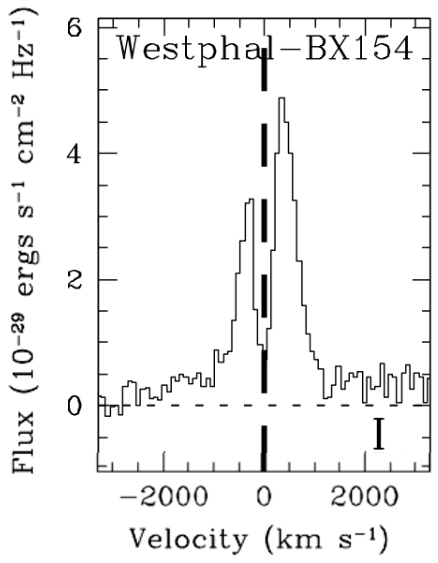
\includegraphics[width=0.3\textwidth]{./figures/kulas_w}
	\end{center}
	\caption{\textbf{Westphal-BX154:} The Kinematics of Multiple-peaked \lya Emission in Star-forming Galaxies at $z\sim2-3$ \cite{Kulas12}. This spectra is at $z=2.5954$.This plot is reproduced with the authors permission.
		\label{fig:kulas_w}}
\end{figure}

TERMINAR...\\

In this model, the combination of rotation and outflows velocities not only makes a lot of sense but seems to be able to fit observations. This new model proposed could replicate \lya profiles with typical LAE's values. The main result of this paper is that we presented a new LAE model roughly consistent with observations.\\


\section{Conclusions}
\label{sec:conclusions}

In this paper, the objective was to analyze and measure the influence of galaxy rotation and outflows on the \lya line. The motivation for this is to be able to obtain physical information of a LAE by just looking at its \lya profile. In order to accomplish this objective, we propose a new model of a LAE consisting of a sphere of Hydrogen atoms that expands radially and rotates as a solid body. The program CLARA \cite{CLARA} is used to set the conditions and emulate the transfer code. \\

The conclusions obtained from this work are: \\

\begin{itemize}
	\item The outgoing spectra depend on the angle an external observer is viewing the galaxy from. The closer it is to the equator of the galaxy, the higher the central valley of the frequency distribution. \\
	
	\item The effects of \vrot, \vout and \tauh are consistent with the different authors that have used them. \vrot broadens the \lya line. \vout increases the peaks asymmetry and \tauh induces a redshift around the zero velocity.\\
	
	\item The final spectra obtained are roughly consistent with LAEs observations.  \\
	
\end{itemize}

\subsection{Future work}

% Rotational effects should be clearly detected and characterized by MUSE.
%Possible rotational velocity constraints using the Lyman-alpha line.


Due to the long time CLARA takes to run, it was not possible to fit an observational LAE and predict its parameters. However, the next step is to use tools as MCMC (Monte Carlo Markov Chain) to obtain the galaxy's \tauh, \vrot and \vout that would agree with this model. \\

TERMINAR...\\

All of this work is available online and free to use to anyone. The data, source code and instructions to replicate this paper's results are in the GitHub repository:  \texttt{github.com/astroandes/CLARA\_RotationOutflows}. \\


\section*{Acknowledgments}

...\\


%------------------------REFERENCES----------------------------

\bibliographystyle{latex/apj}
\bibliography{references}

%------------------------APPENDIX----------------------------

\newpage

\appendix

\begin{figure}[!htbp]
	\centering
	\begin{minipage}[b]{0.45\textwidth}
		\section{Results' Figures}
		\label{ap:results_figures}
		
		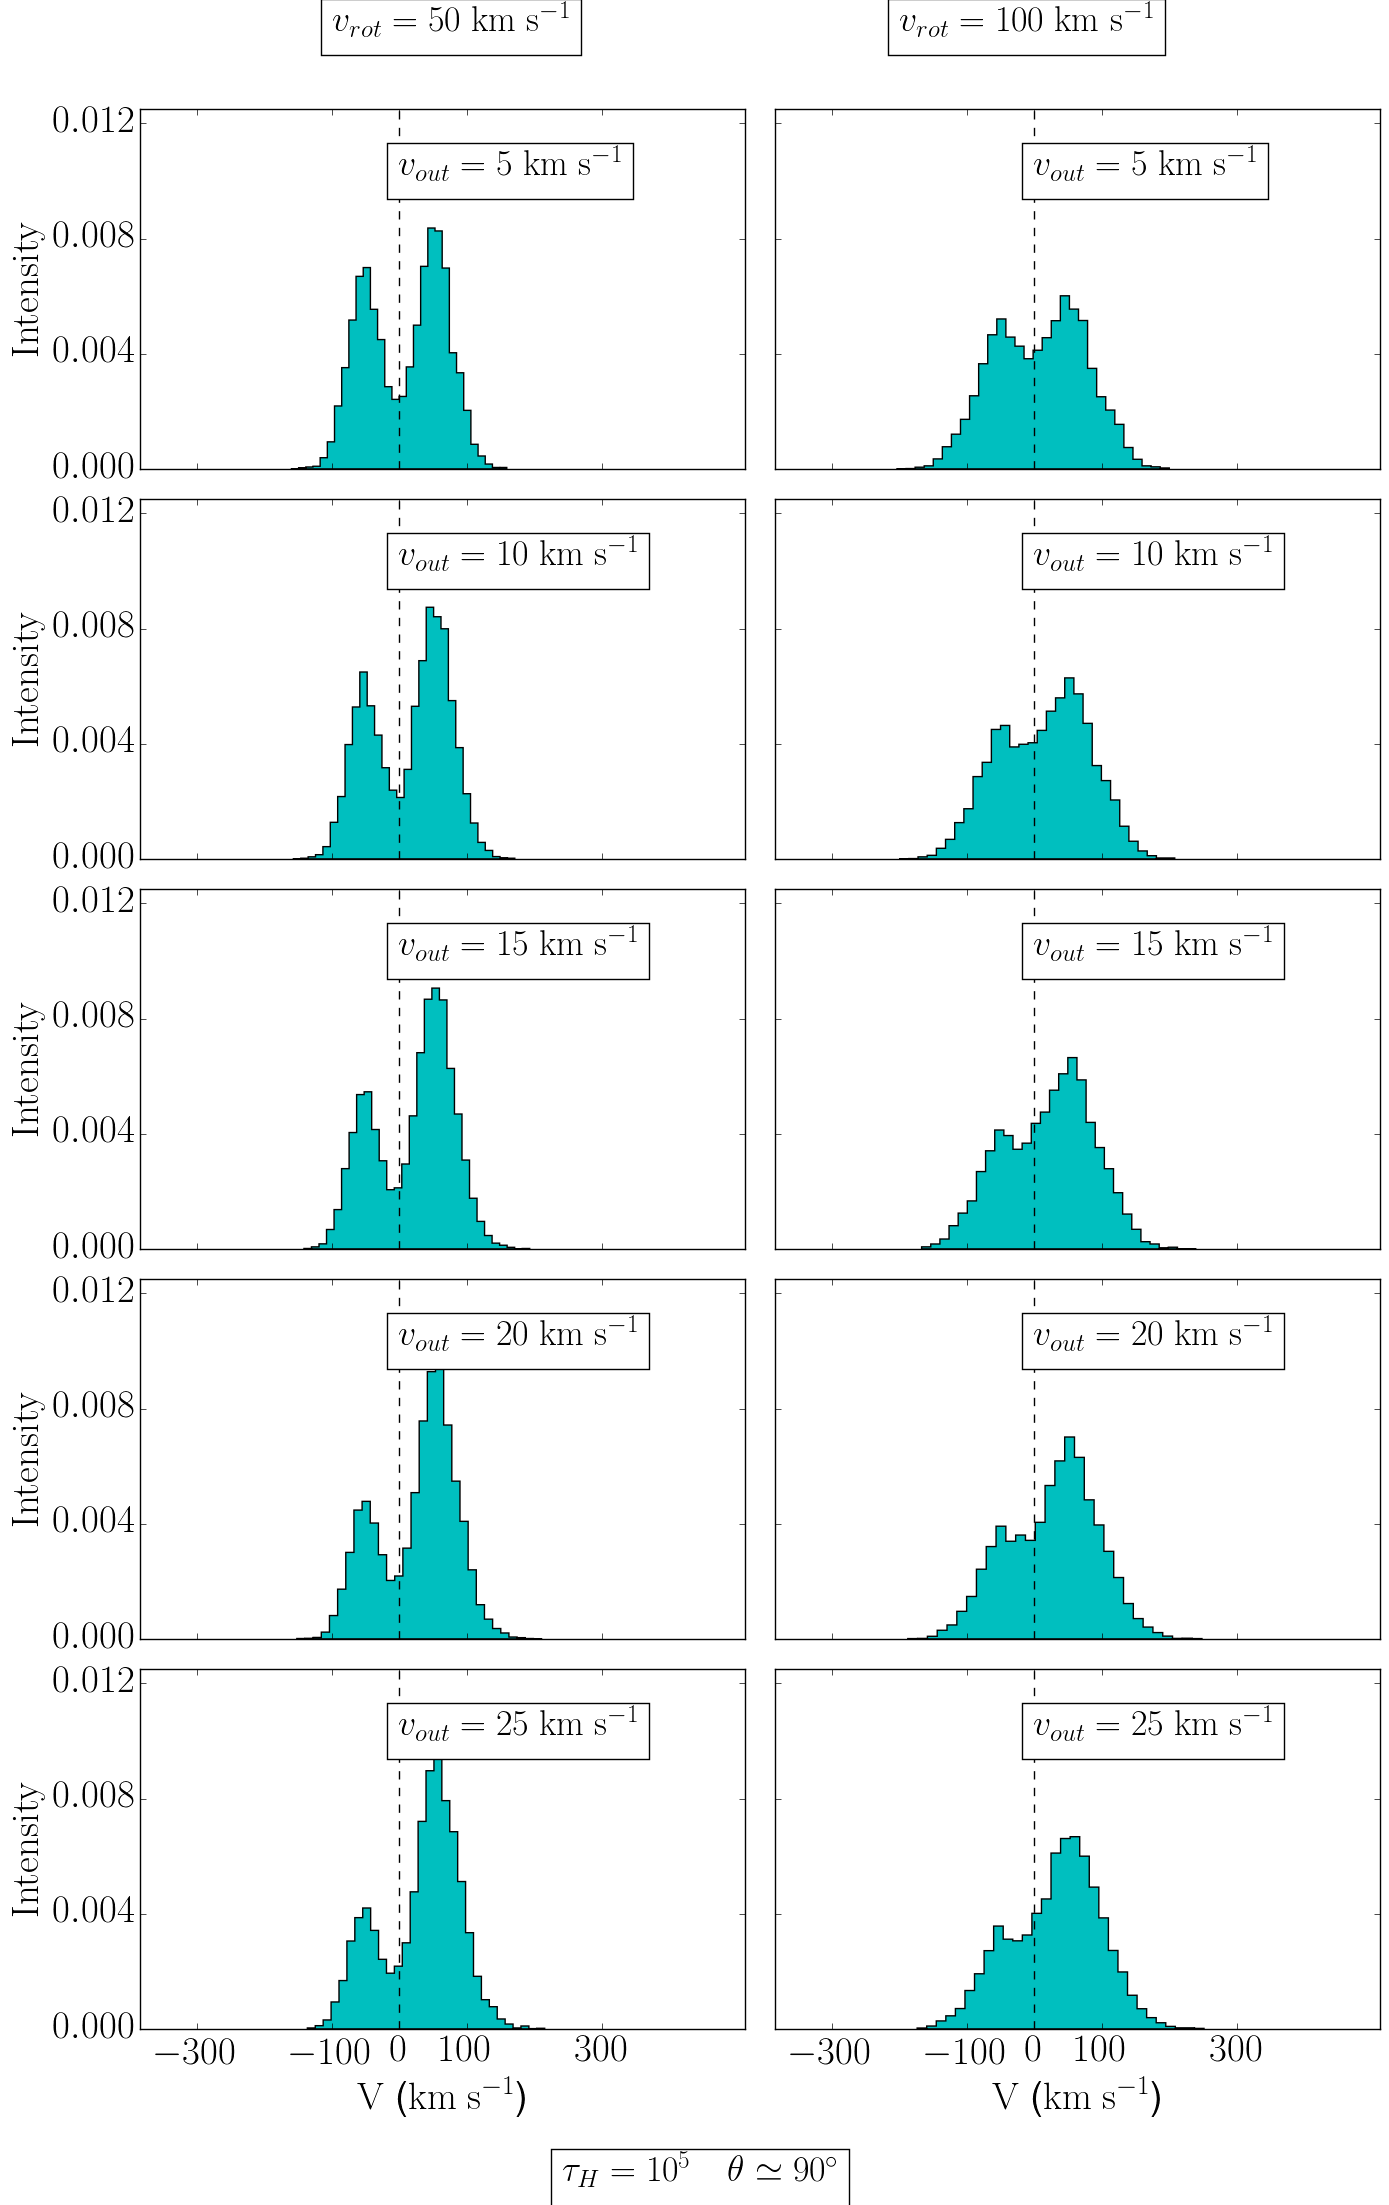
\includegraphics[width=\textwidth]{./figures/3_tau10E5_phi83-90}
		\caption{\textbf{\lya profile for \tauh$=10^5$:} With \vrot ranging $50,100$ \kms and \vout ranging $5,10,15,20,25$ \kms. The intensity is in arbitrary units. The viewing angle $\theta \simeq 90^\circ$. The dashed vertical line indicates the \lya line's natural frequency. 
			\label{fig:3_tau10E5_phi83-90}}
	\end{minipage}
	\hfill
	\begin{minipage}[b]{0.45\textwidth}
		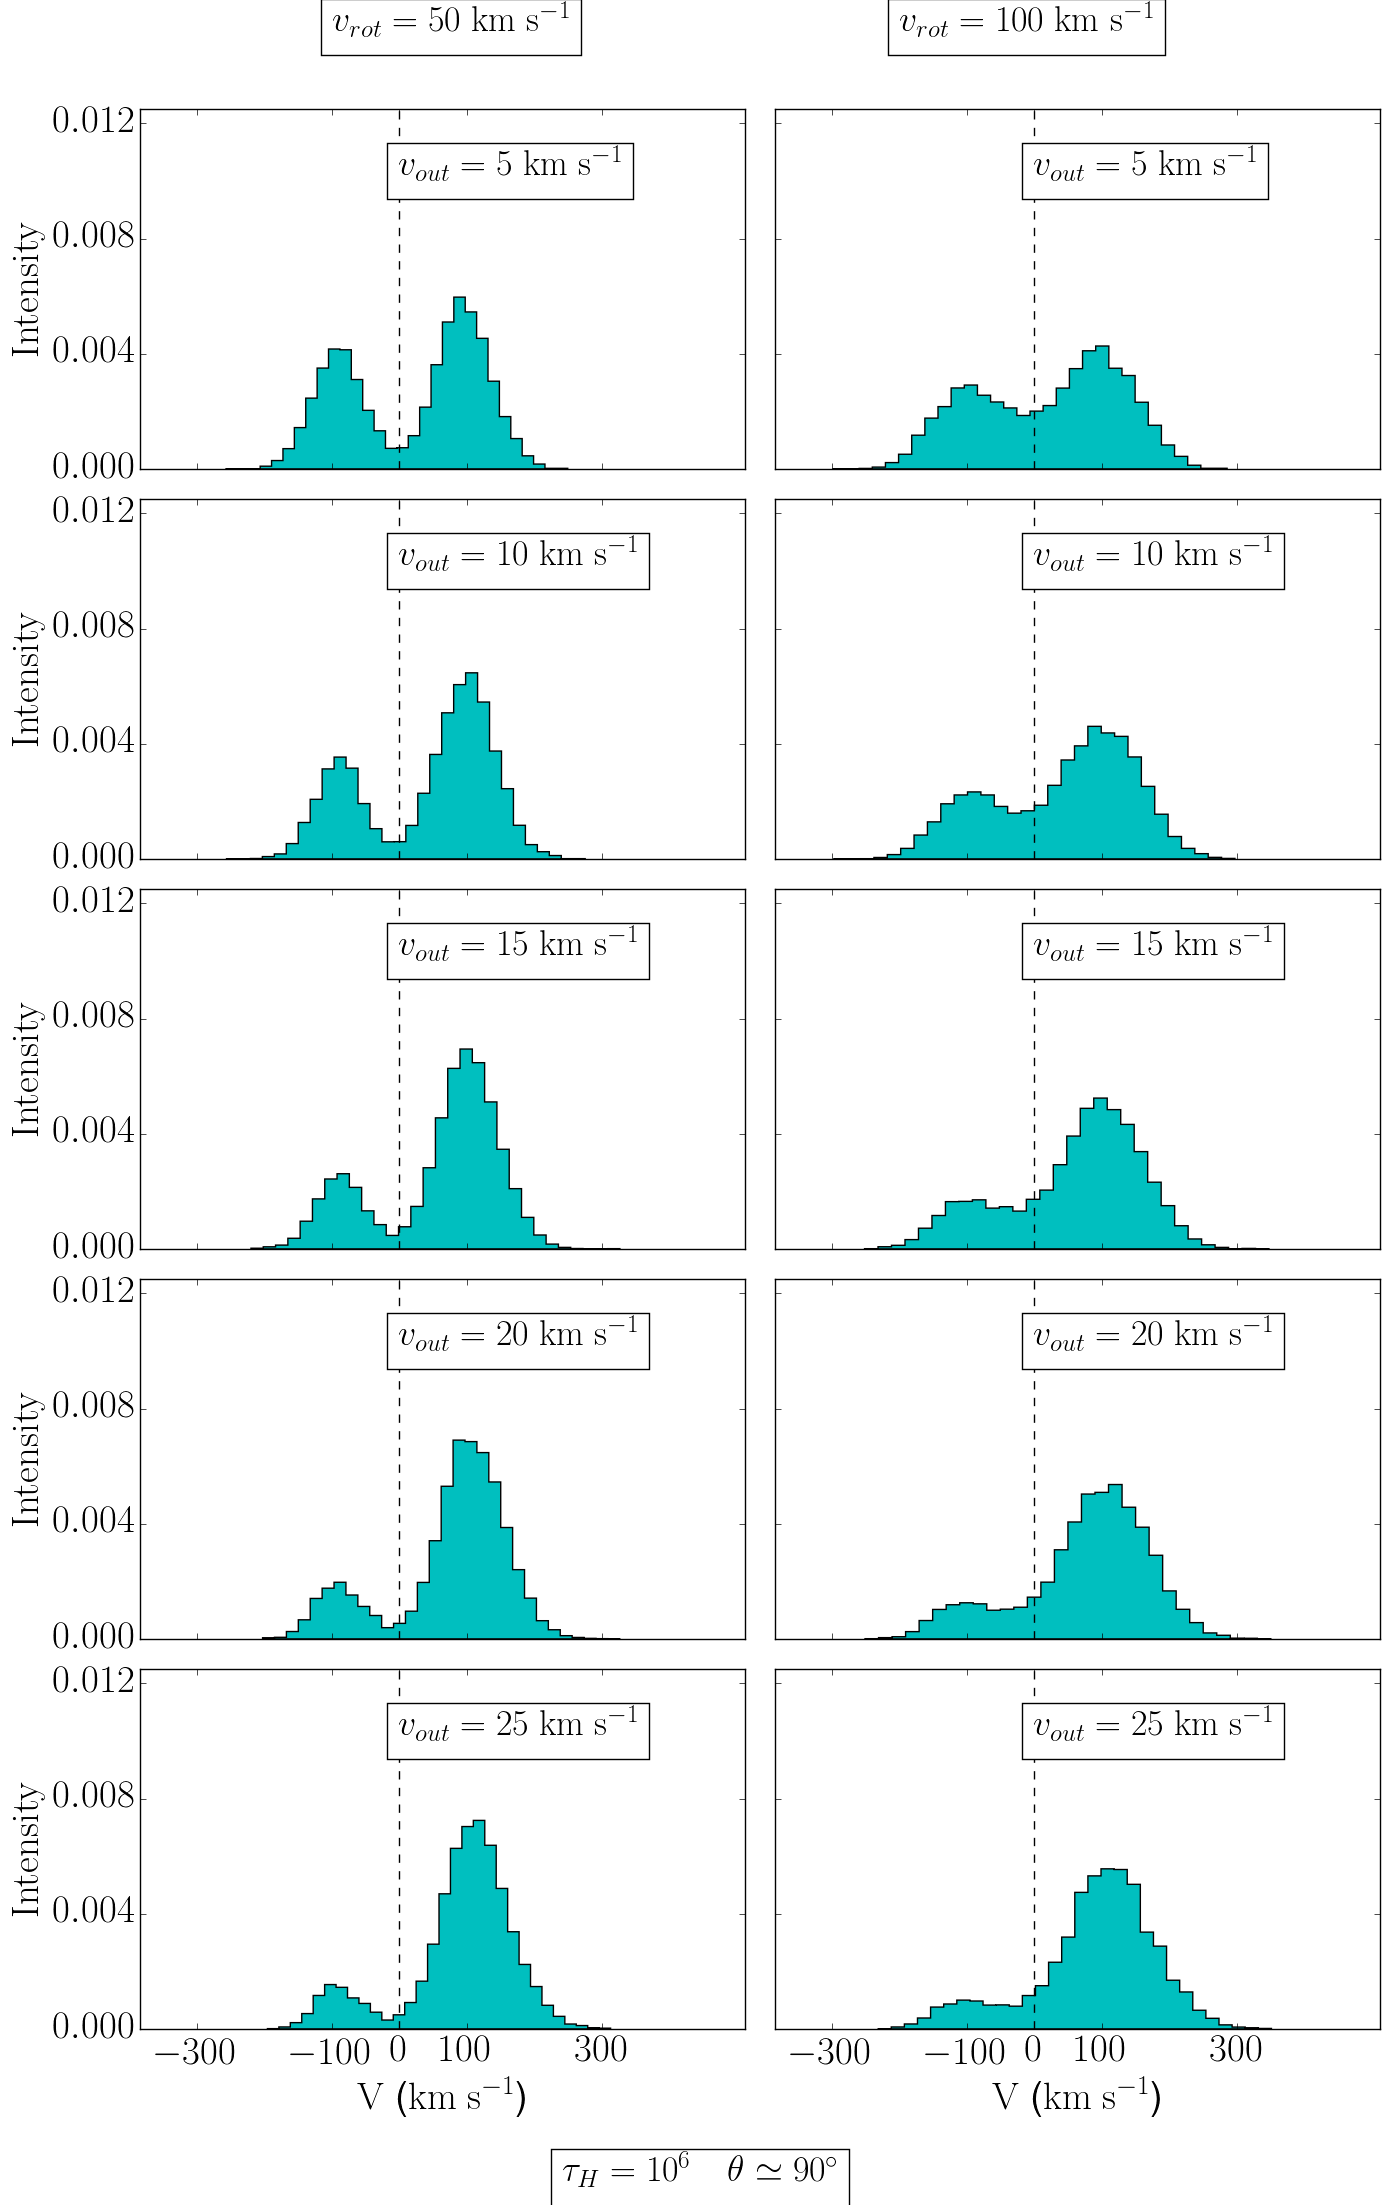
\includegraphics[width=\textwidth]{./figures/3_tau10E6_phi83-90}
		\caption{\textbf{\lya profile for \tauh$=10^6$:}  Same as Fig. \ref{fig:3_tau10E5_phi83-90} but for \tauh$=10^6$. 
			\label{fig:3_tau10E6_phi83-90}}
		\vspace{1.5mm}
	\end{minipage}
\end{figure}

\begin{figure}[!htbp]
	\centering
	\begin{minipage}[b]{0.45\textwidth}
		\vspace{3mm}
		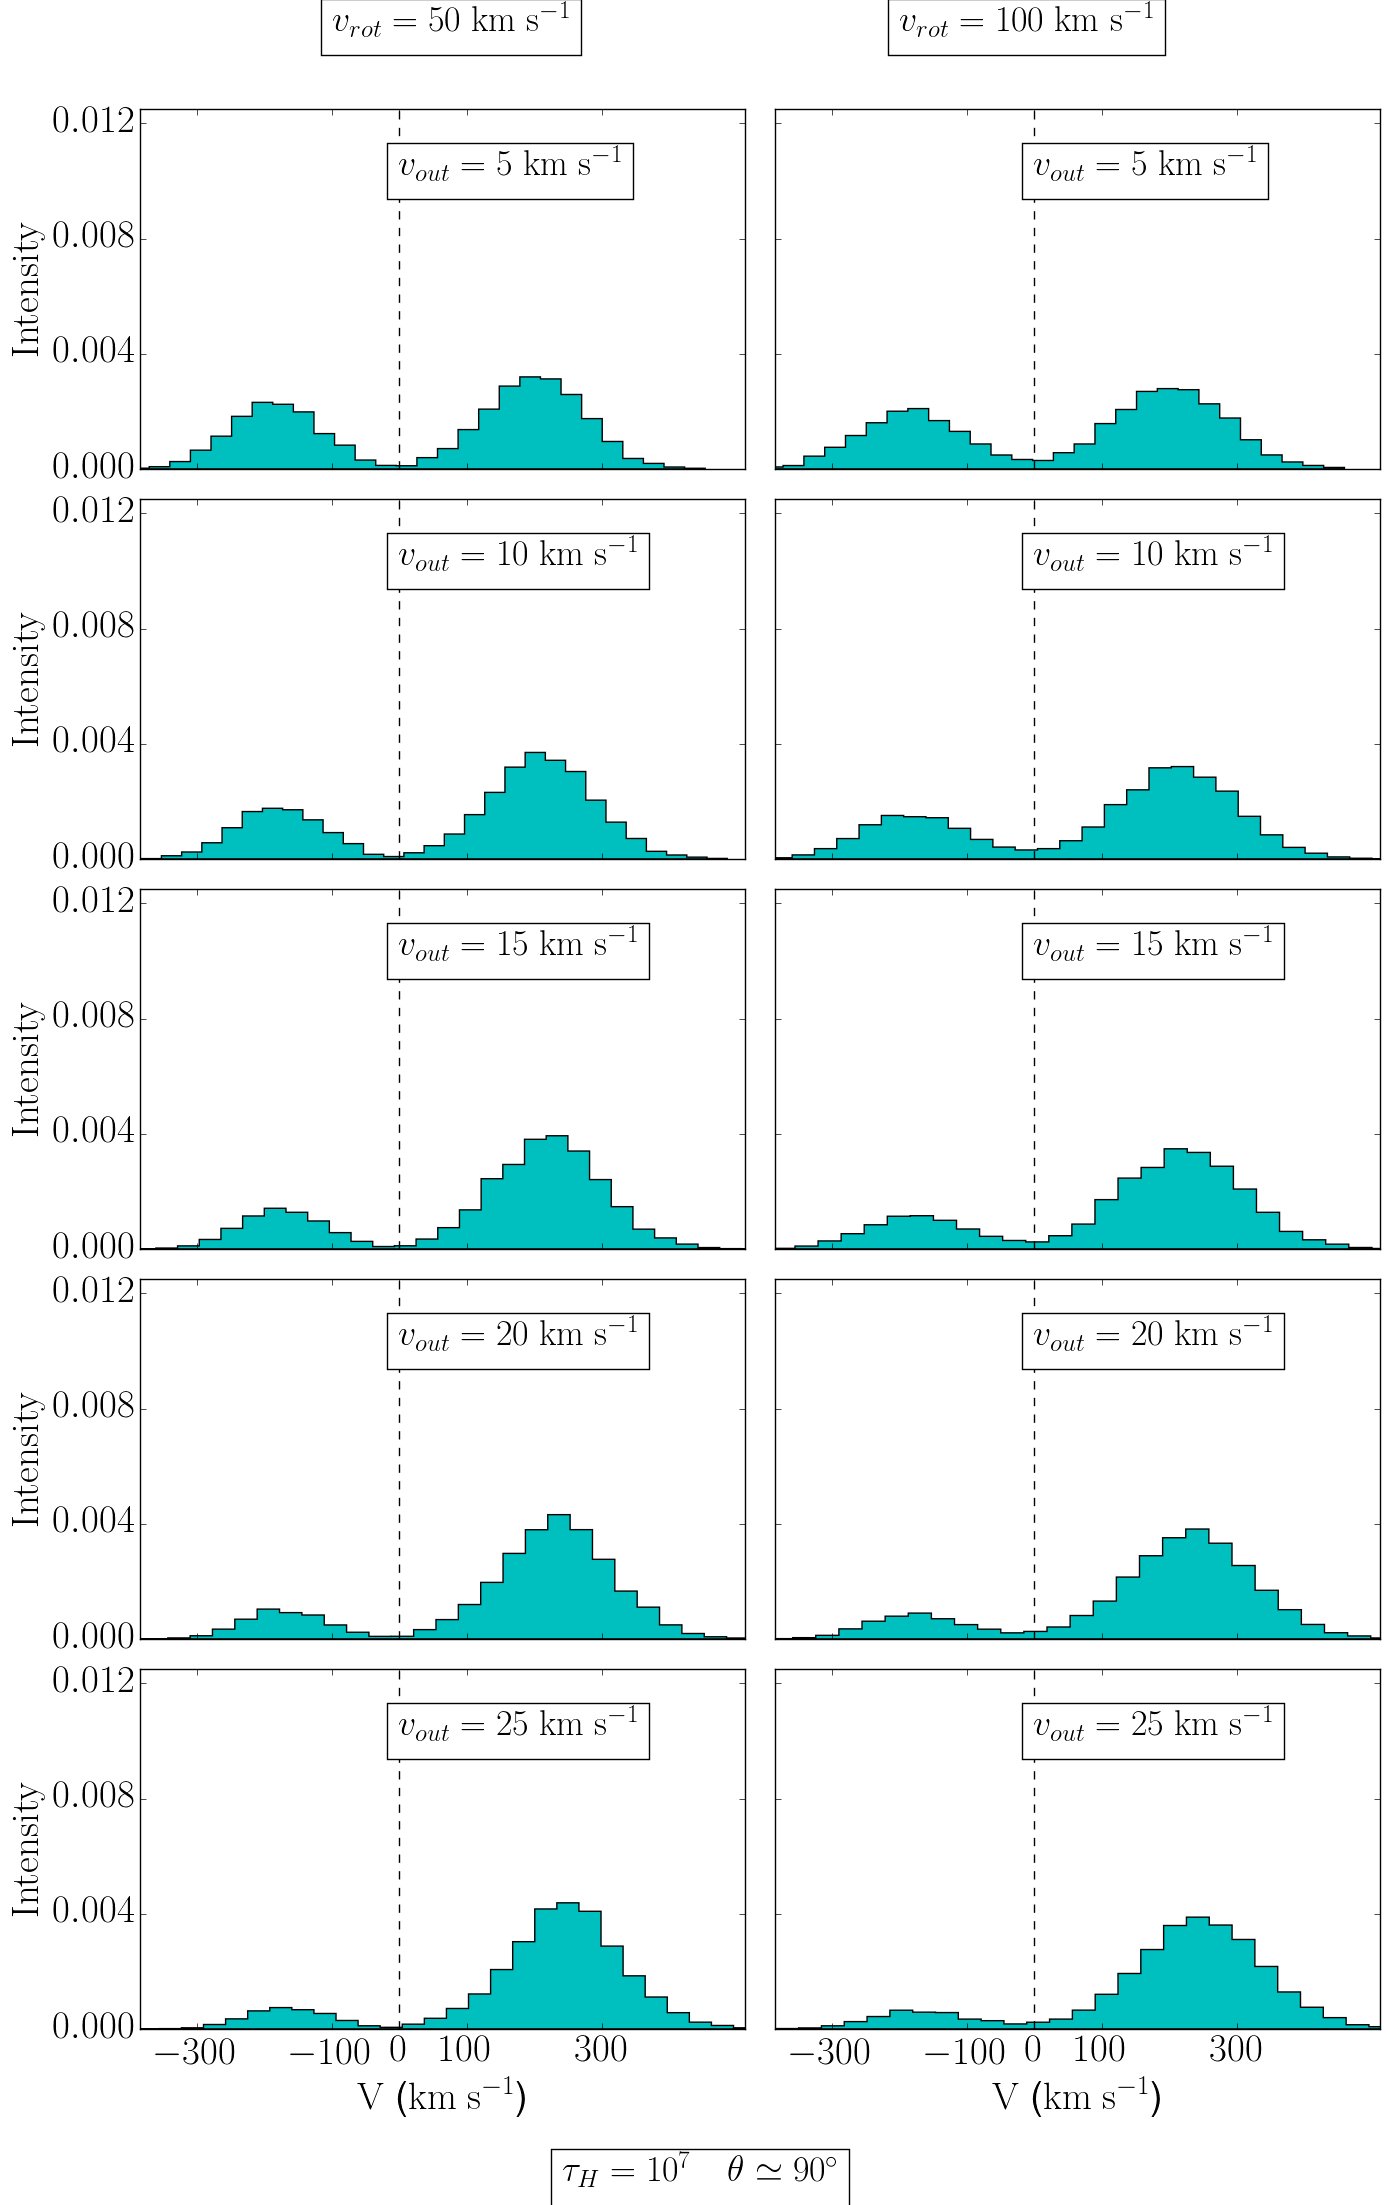
\includegraphics[width=\textwidth]{./figures/3_tau10E7_phi83-90}
		\caption{\textbf{\lya profile for \tauh$=10^7$:} Same as Fig. \ref{fig:3_tau10E5_phi83-90} but for \tauh$=10^7$.
			\label{fig:3_tau10E7_phi83-90}}
	\end{minipage}
	\hfill
	\begin{minipage}[b]{0.45\textwidth}
		\section{Additional Figures}
		\label{ap:additional_figures}
		
		Additional figures of spectra with \vrot $= 50,100$ \kms and \vout $= 50,75$ \kms, for all the different \tauh. 
		
		\vspace{2.7cm}
		
		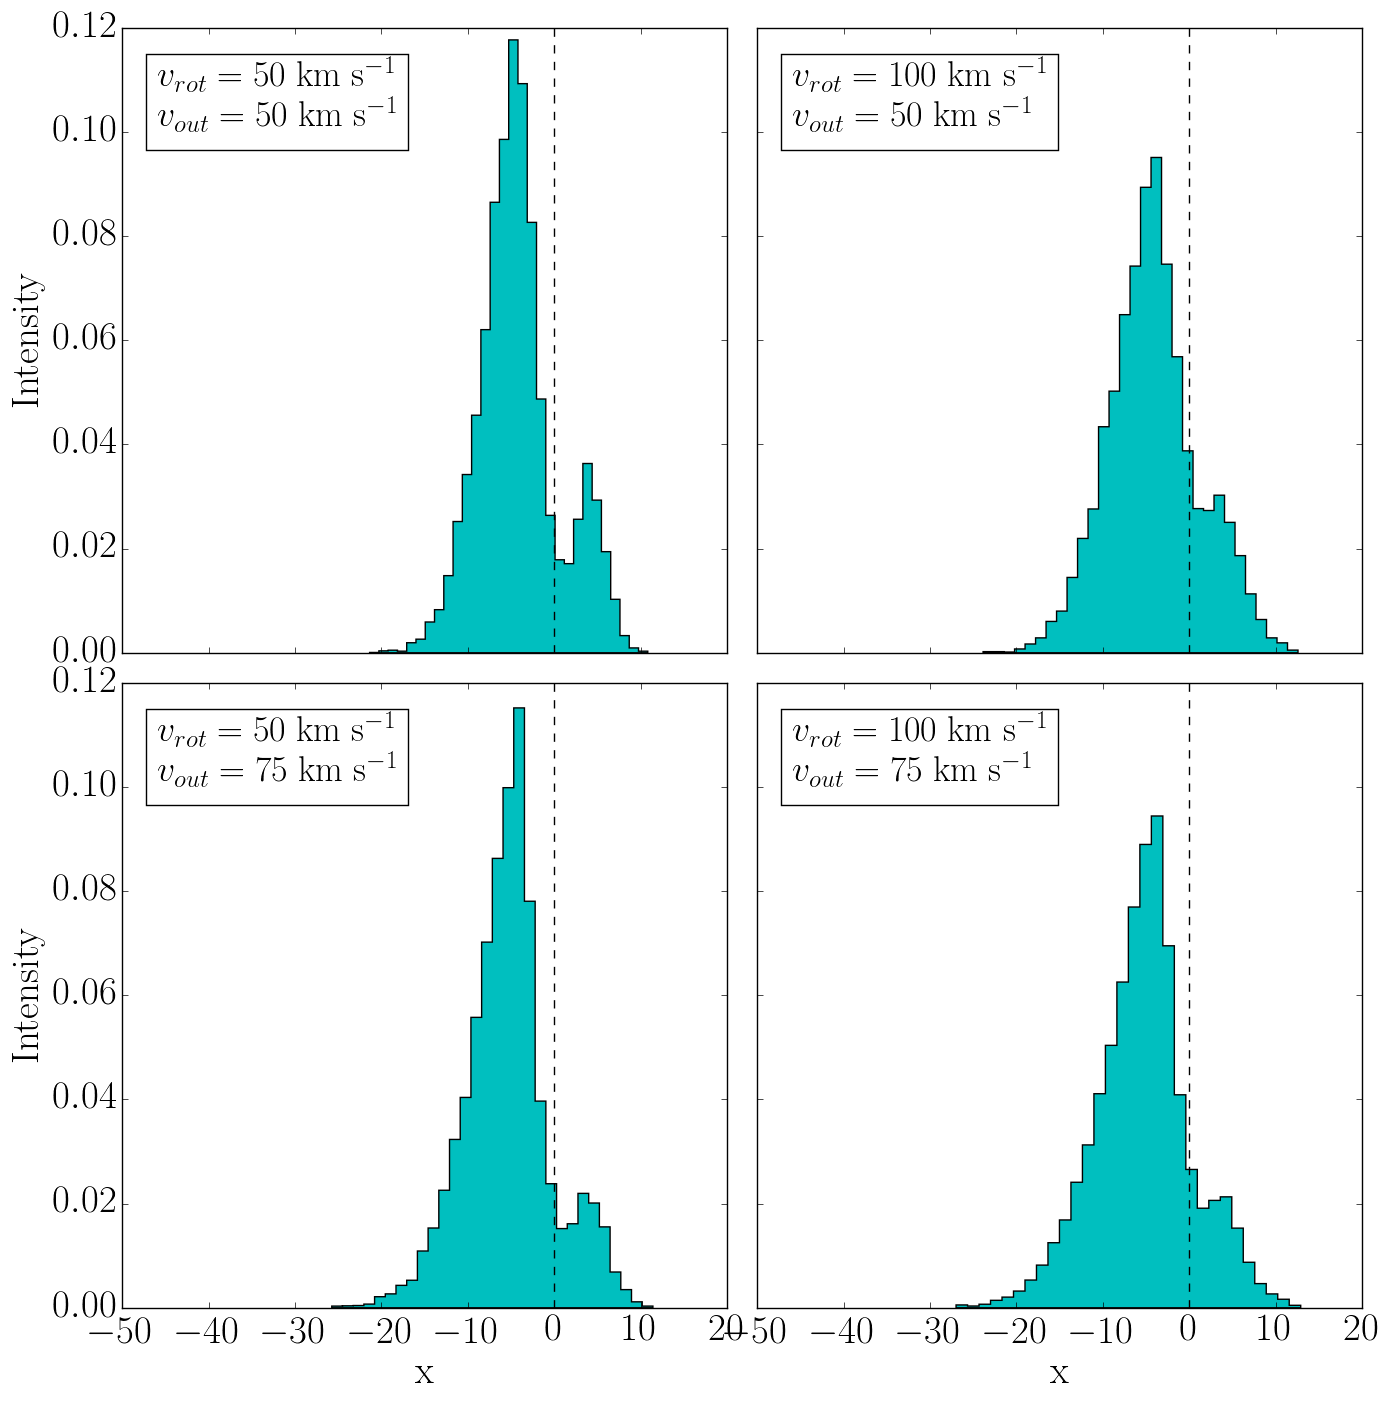
\includegraphics[width=\textwidth]{./figures/appendix/2_tau10E5_phi83-90}
		\caption{\textbf{\lya profile for \tauh$=10^5$:} With \vrot ranging $50,100$ \kms and \vout ranging $50,75$ \kms.
			\label{fig:2_tau10E5_phi83-90}}
	\end{minipage}
\end{figure}

\begin{figure}[!htbp]
	\centering
	\begin{minipage}[b]{0.45\textwidth}
		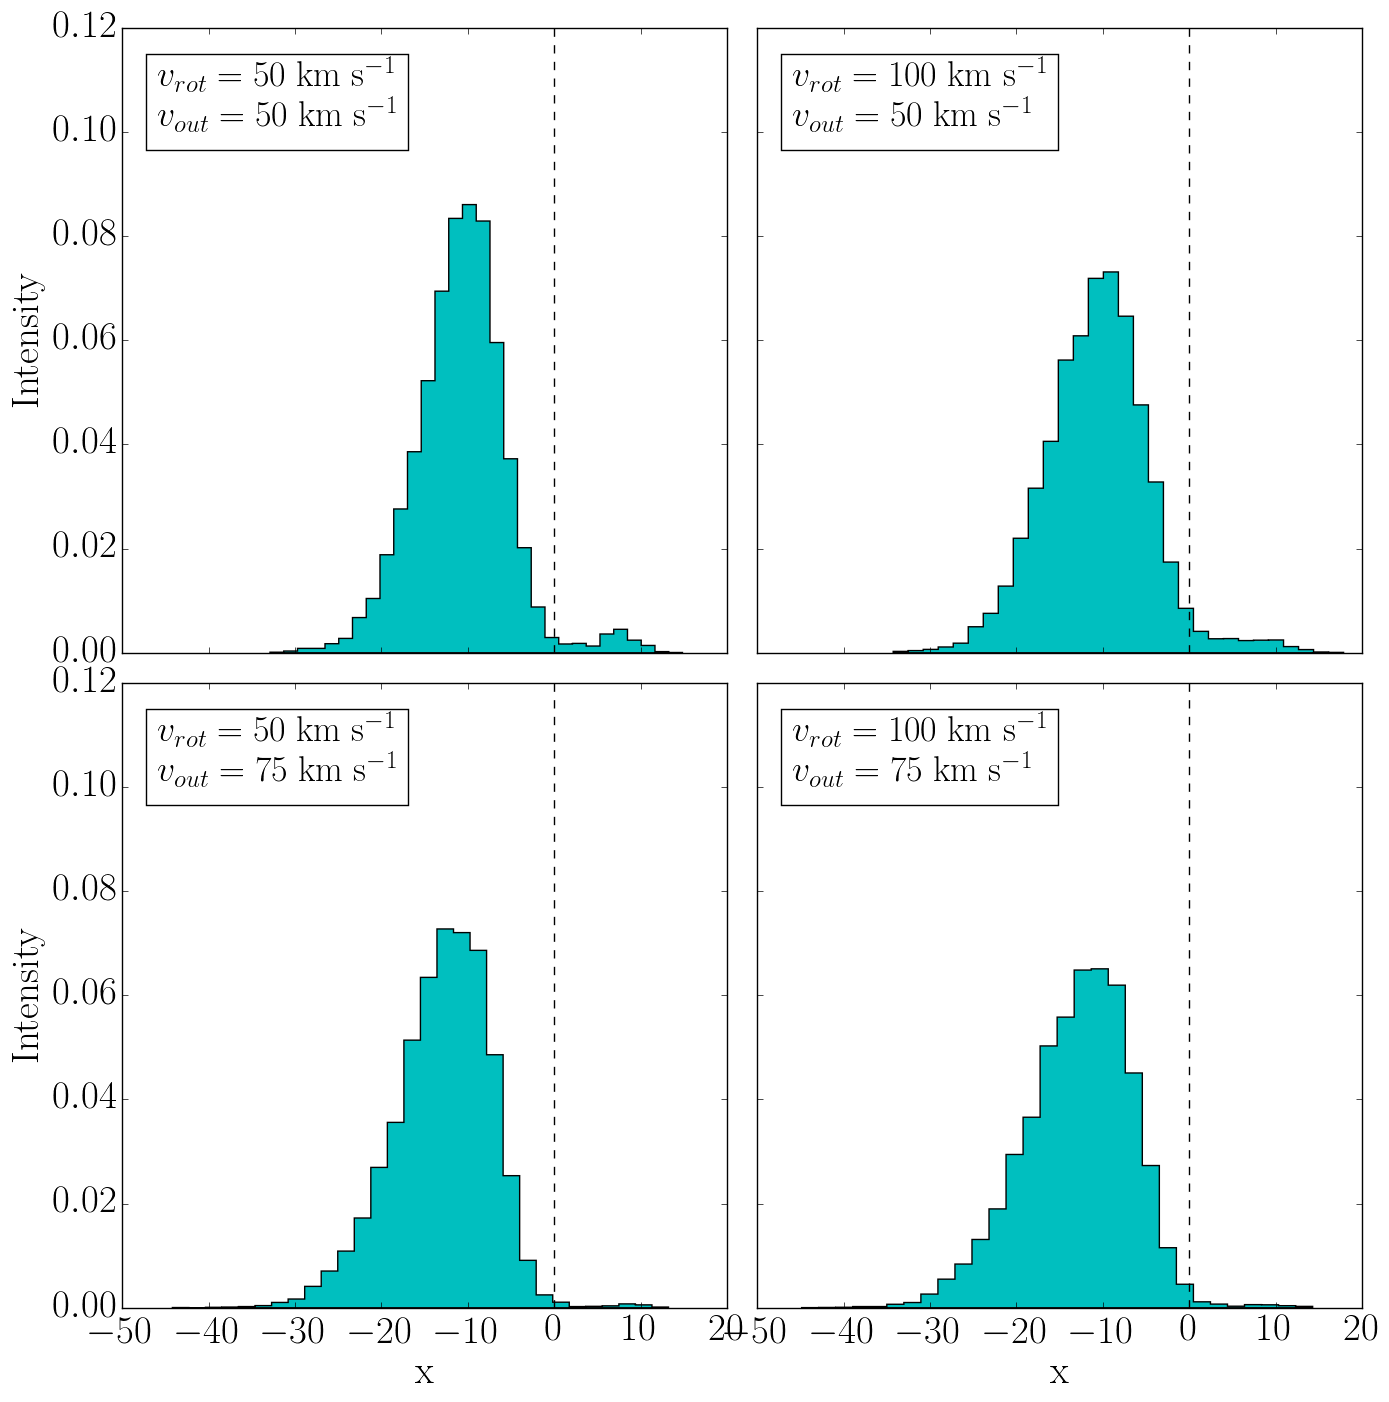
\includegraphics[width=\textwidth]{./figures/appendix/2_tau10E6_phi83-90}
		\caption{\textbf{\lya profile for \tauh$=10^6$:} With \vrot ranging $50,100$ \kms and \vout ranging $50,75$ \kms.
			\label{fig:2_tau10E6_phi83-90}}
	\end{minipage}
	\hfill
	\begin{minipage}[b]{0.45\textwidth}
		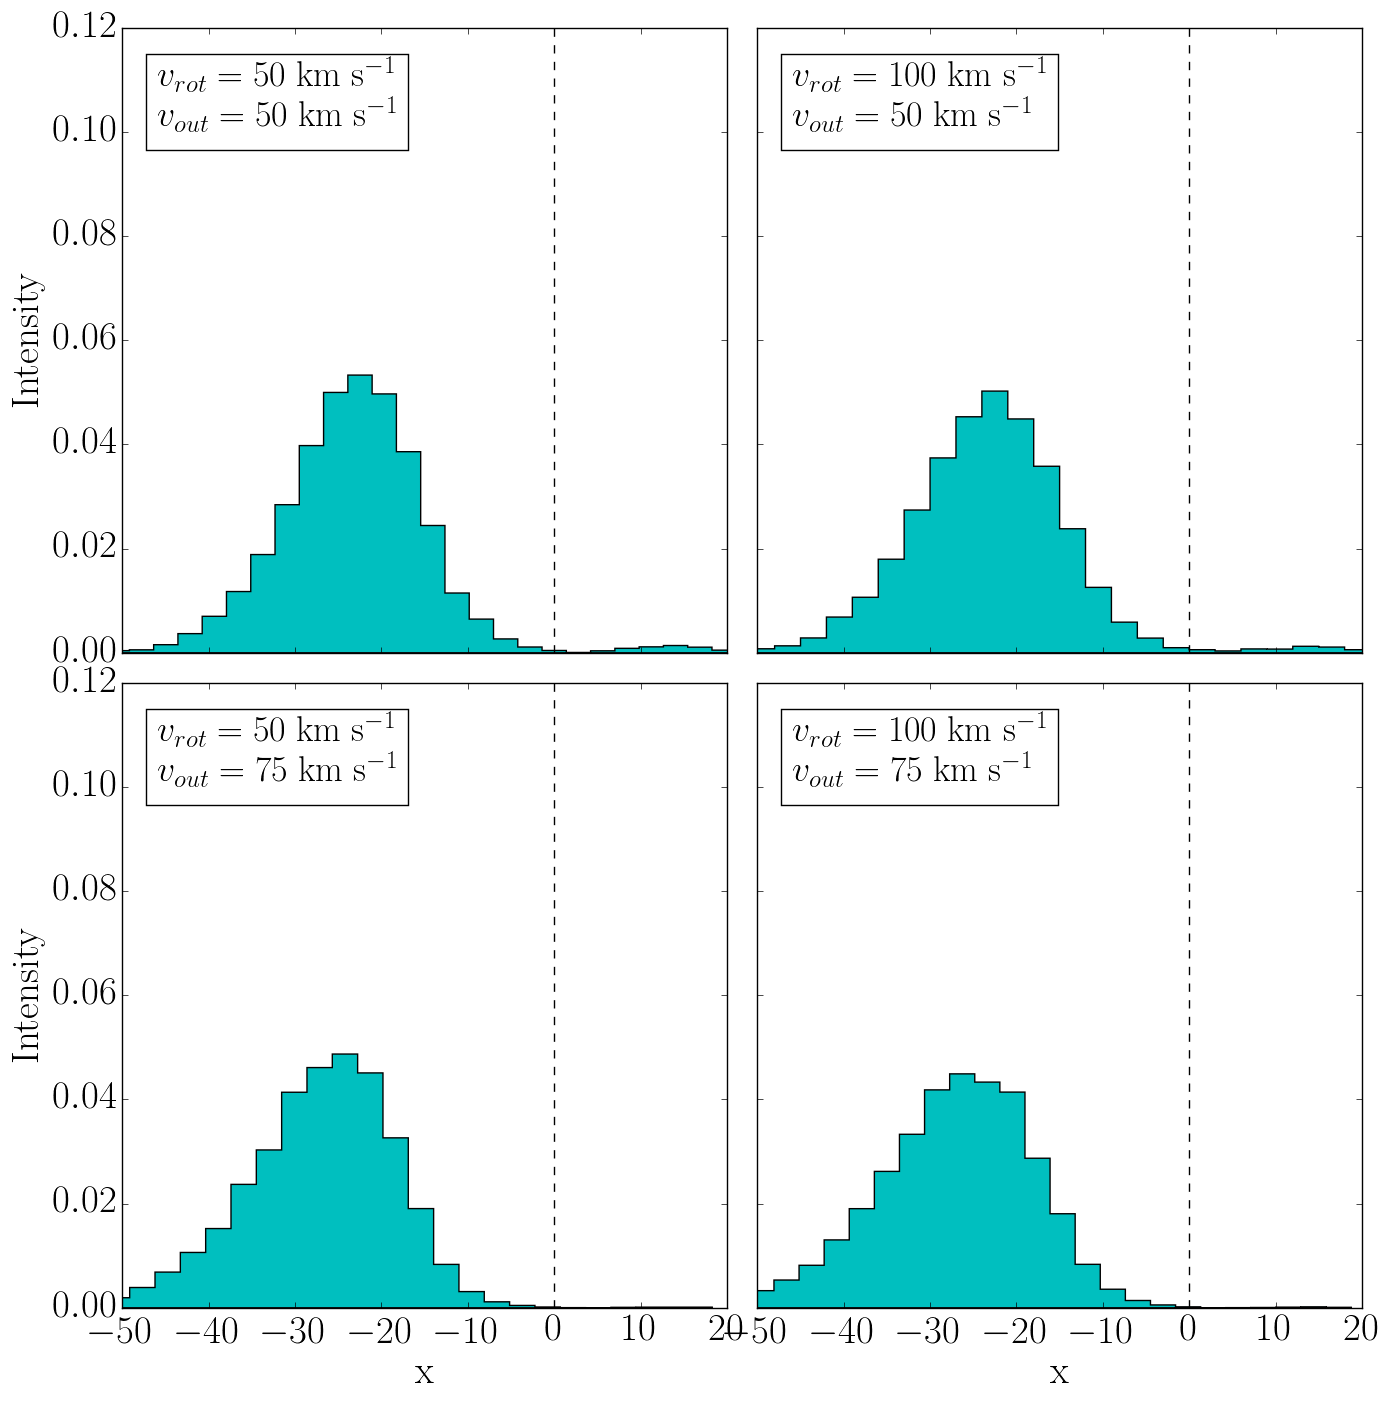
\includegraphics[width=\textwidth]{./figures/appendix/2_tau10E7_phi83-90}
		\caption{\textbf{\lya profile for \tauh$=10^7$:} With \vrot ranging $50,100$ \kms and \vout ranging $50,75$ \kms.
			\label{fig:2_tau10E7_phi83-90}}
	\end{minipage}
\end{figure}

\end{document}